%%%%%%%%%%%%%%%%%%%%%%%%%%%%%%%%%%%%%%%%%
% Journal Article
% LaTeX Template
% Version 2.0 (February 7, 2023)
%
% This template originates from:
% https://www.LaTeXTemplates.com
%
% Author:
% Vel (vel@latextemplates.com)
%
% License:
% CC BY-NC-SA 4.0 (https://creativecommons.org/licenses/by-nc-sa/4.0/)
%
% NOTE: The bibliography needs to be compiled using the biber engine.
%
%%%%%%%%%%%%%%%%%%%%%%%%%%%%%%%%%%%%%%%%%

%----------------------------------------------------------------------------------------
%	PACKAGES AND OTHER DOCUMENT CONFIGURATIONS
%----------------------------------------------------------------------------------------

\documentclass[
  a4paper, % Paper size, use either a4paper or letterpaper
  10pt, % Default font size, can also use 11pt or 12pt, although this is not recommended
  unnumberedsections, % Comment to enable section numbering
  twoside, % Two side traditional mode where headers and footers change between odd and even pages, comment this option to make them fixed
]{LTJournalArticle}

\addbibresource{sample.bib} % BibLaTeX bibliography file

\runninghead{Praxisprojekt: Quantenalgorithmen, Juli 2023} % A shortened article title to appear in the running head, leave this command empty for no running head

\footertext{} % Text to appear in the footer, leave this command empty for no footer text

\setcounter{page}{1} % The page number of the first page, set this to a higher number if the article is to be part of an issue or larger work

\usepackage[braket, qm]{qcircuit}
\usepackage{graphicx}
\usepackage{hyperref}
\usepackage{physics}
\usepackage{graphicx}
\graphicspath{{./pictures/}}

\hypersetup{
  colorlinks=true,
  linkcolor=blue,
  filecolor=magenta,    
  urlcolor=blue,
  pdftitle={Praxisprojekt: Quantenalgorithmen, Juli 2023},
  pdfpagemode=FullScreen,
}

\usepackage[ngerman]{babel}
\DeclareMathOperator{\Landau}{\mathcal{O}} % Landau/Big-O Notation


%----------------------------------------------------------------------------------------
%	TITLE SECTION
%----------------------------------------------------------------------------------------

\title{Implementierung einer Bibliothek von Quantenalgorithmen zur Kryptoanalyse} % Article title, use manual lines breaks (\\) to beautify the layout

% Authors are listed in a comma-separated list with superscript numbers indicating affiliations
% \thanks{} is used for any text that should be placed in a footnote on the first page, such as the corresponding author's email, journal acceptance dates, a copyright/license notice, keywords, etc
\author{%
  Simon Kalytta\textsuperscript{1,2}, Janis König\textsuperscript{2}
}

% Affiliations are output in the \date{} command
\date{%
  \footnotesize\textsuperscript{\textbf{1}}%
  Fachhochschule Aachen, 
  Eupener Str. 70, 52066 Aachen\\
  \textsuperscript{\textbf{2}}%
  it.sec GmbH,
  Einsteinstr. 55, 89077 Ulm%
}

% Full-width abstract
\renewcommand{\maketitlehookd}{%
  \begin{abstract}
    \noindent
    Seit der Entwicklung des theoretischen Konzepts eines Quantencomputers in den 1980er Jahren
    wurden Quantenalgorithmen entworfen,
    die durch die Ausnutzung der Quantenmechanik bestimmte Berechnungen effizienter lösen können
    als die schnellsten bekannten klassischen Algorithmen.
    Insbesondere betreffen sie mathematische Probleme,
    die die Grundlage aktueller kryptografischer Verfahren bilden.
    Obwohl derzeit keine Quantencomputer mit ausreichender Rechenleistung existieren,
    hat die Entwicklung in den letzten Jahren an Geschwindigkeit gewonnen und
    sollte aufgrund der erwarteten zukünftigen Fortschritte in der IT-Sicherheit berücksichtigt werden.

    Um eine Grundlage für die zukünftige Anwendung von Quantenalgorithmen zu schaffen,
    wird eine eigene Bibliothek mit den bekanntesten Quantenalgorithmen entwickelt.
    Die Implementierungen umfassen ressourcensparende Varianten,
    die gleichzeitig skalierbar sind,
    um mit leistungsstärkeren Quantencomputern umfangreichere Eingabegrößen zu bewältigen.
    Derzeit gibt es nur wenige praktische Umsetzungen von Quantenalgorithmen und
    noch weniger spezifische Implementierungen für die Kryptoanalyse.
    Eine genauere Untersuchung von Quantenalgorithmen und
    deren Auswirkung auf unsere Kryptografie
    wird jedoch mit fortschreitender Leistungsfähigkeit von Quantencomputern immer wichtiger.
  \end{abstract}
}

%----------------------------------------------------------------------------------------





\begin{document}

\maketitle % Output the title section

%----------------------------------------------------------------------------------------
%	ARTICLE CONTENTS
%----------------------------------------------------------------------------------------

\subsection{Einleitung}

Heutzutage hat nahezu jeder schon einmal von Quantencomputern gehört.
Allerdings beschränkt sich das Wissen über diese Technologie oft lediglich auf den Begriff selbst.
Selbst Personen aus der IT-Branche verbinden mit einem Quantencomputer häufig nur
eine neuartige Zukunftstechnologie eines besonders leistungsfähigen Supercomputers nach der von-Neumann-Architektur.

Die ersten Ansätze zur Entwicklung von Quantencomputern gehen jedoch bereits auf die 1980er Jahre zurück,
als der Physiker Richard Feynman feststellte,
dass klassische Computer Schwierigkeiten haben würden,
bestimmte quantenphysikalische Phänomene nachzubilden.
Feynman kam zu dem Schluss, dass ein Computer,
der nach den Gesetzen der Quantenmechanik arbeitet,
möglicherweise besser geeignet wäre,
quantenmechanische Systeme zu simulieren~\autocite{Feynman:1982}.
Erst mehr als ein Jahrzehnt später, im Jahr 1998,
gelang die erste physikalische Realisierung eines Quantencomputers
mit insgesamt zwei Qubits~\autocite{Chuang:1998ExperimentalIO}.

Seitdem hat sich die Entwicklungsgeschwindigkeit deutlich erhöht,
insbesondere aufgrund des Engagements großer Unternehmen wie IBM, Microsoft, Google und Intel.
Ein Beispiel dafür ist IBM,
das seit der Vorstellung ihres 27-Qubits-Systems namens "`Falcon"'
eine jährliche Verdoppelung der vorhandenen Qubits bei ihren neuen Systemen plant.
Bislang konnte dieser Trend aufrechterhalten werden
indem im Jahr 2022 IBM mit ihrem "`Osprey"'-System 433~Qubits erreichte~\autocite{IBM:2022}.
Basierend auf den Fortschritten der letzten Jahre und
den Prognosen für die kommenden Jahre erwartet
das Bundesamt für Sicherheit in der Informationstechnik,
dass in den 2030er Jahren Quantencomputer existieren werden,
die für die Kryptografie relevant sein werden~\autocite{BSI:2023}.
In diesem Zusammenhang sind insbesondere zwei Anwendungsbereiche für die Kryptografie von Bedeutung:
zum einen die Quantenkryptografie, bei der die Eigenschaften der Quantenmechanik genutzt werden,
um Sicherheit in der Kommunikation zu gewährleisten, und
zum anderen die Kryptoanalyse mit Quantenalgorithmen, die darauf abzielt,
Verschlüsselungsverfahren zu schwächen oder sogar vollständig zu brechen.

Trotz einiger theoretischer Arbeiten zu Quantenalgorithmen
besteht immer noch eine deutliche Lücke in Bezug auf praktische Ansätze mit Fokus auf die Kryptoanalyse.
Daher bietet es sich an, diese Lücke zu schließen und die Funktionsweise solcher Algorithmen genauer zu untersuchen.
Das Ziel dieser Arbeit besteht darin, eine Bibliothek zur Kryptoanalyse zu entwickeln,
die aktuelle Verschlüsselungsverfahren mithilfe von Quantenalgorithmen kompromittiert.
Um sicherzustellen, dass die Bibliothek auch mit zukünftigen Quantencomputern kompatibel ist,
skalieren die Implementierungen mit zusätzlichen Qubits und
ermöglichen so die Verarbeitung komplexerer Eingabegrößen.

Die Realisierung erfolgt in Python unter Verwendung des Softwareentwicklungskits Qiskit.
Qiskit ist ein Open-Source-SDK von IBM,
das speziell für die Entwicklung von Anwendungen für Quantencomputer entwickelt wurde.
Programme, die mithilfe von Qiskit entwickelt wurden,
können über die Cloud auf den Quantencomputern von IBM getestet werden.
Aufgrund der begrenzten Rechenleistung der derzeit verfügbaren kostenlosen Quantensysteme
werden die Implementierungen mithilfe von Simulatoren getestet.


%------------------------------------------------

\subsection{Stand der Technik}

Für die Kryptoanalyse mit Quantencomputern spielen zwei Quantenalgorithmen eine besonders wichtige Rolle:

\subsubsection{Shor-Algorithmus}
Der Shor-Algorithmus ist ein quantenbasiertes Verfahren,
das die Primfaktorzerlegung und die Berechnung des diskreten Logarithmus
mit polynomialem Aufwand bewältigen kann.
Da es für beide dieser Berechnungen keinen effizienten klassischen Algorithmus gibt,
spielen sie eine essentielle Rolle in der Kryptografie~\autocite{Shor:1997}.
Zahlreiche theoretische Arbeiten beschäftigen sich mit dem Shor-Algorithmus und
insbesondere mit der Optimierung zur Reduktion der benötigten Qubits.

Im Bereich praktischer Umsetzungen und Realisierungen
gibt es bisher keine skalierbare Implementierung des Shor-Algorithmus in Qiskit.
Die meisten praktischen Umsetzungen bedienen sich einer vereinfachten Variante,
die ausschließlich die Faktorisierung der Zahl 15 ermöglicht.
Dadurch ist die Schaltung einfach nachzustellen,
und die Funktionsweise des Algorithmus kann dennoch demonstriert werden~\autocite{9376169, Monz_2016, IBM:Shor}.

In der Vergangenheit gab es eine skalierbare Version des Shor-Algorithmus in Qiskit.
Diese ist jedoch nicht mehr importierbar und als veraltet gekennzeichnet.
In der Dokumentation findet man noch immer einen entsprechenden Eintrag.
Dort kann man nachlesen, dass die damals implementierte Version eine Variante war,
die \(4n+2\) Qubits erforderte~\autocite{IBM:Shor_docu}.

\subsubsection{Grover-Algorithmus}
Der Grover-Algorithmus ist ein quantenbasiertes Suchverfahren,
das eine quadratische Geschwindigkeitsverbesserung
gegenüber dem besten klassischen Suchalgorithmus bietet~\autocite{grover1996fast}.
Der Algorithmus ermöglicht die effiziente Suche in unsortierten Datenbanken.
In Bezug auf die Kryptoanalyse bedeutet dies,
dass mithilfe des Grover-Algorithmus der Gesamtraum aller möglichen Schlüssel
eines Verschlüsselungsverfahrens effizienter nach einem passenden Schlüssel durchsucht werden kann.

Konkret bedeutet dies,
dass der Grover-Algorithmus eine deutliche Verbesserung gegenüber dem besten klassischen Suchalgorithmus bietet,
der eine lineare Laufzeit aufweist.
Die Laufzeit des Grover-Algorithmus beträgt \(\Landau(\sqrt N)\),
wobei \(N\) für die Anzahl der Elemente in der Datenbank steht,
im Vergleich zur linearen Laufzeit \(\Landau(N)\) des klassischen Suchalgorithmus.
Im Fall des Verschlüsselungsverfahrens AES-128 würde dies bedeuten,
dass die Laufzeit von \(\Landau(2^{128})\) auf \(\Landau(2^{64})\) reduziert wird.

Es wurden verschiedene Arbeiten zur praktischen Umsetzung des Grover-Algorithmus durchgeführt.
Einige dieser Arbeiten wurden auch mit Hilfe von Qiskit umgesetzt,
und Qiskit bietet eine importierbare Implementierung des Algorithmus~\autocite{IBM:Grover}.

Aufgrund der Natur des Grover-Algorithmus ist für die Kryptoanalyse ein Orakel erforderlich,
das erkennt, ob ein gegebenes Ergebnis eine gültige Lösung darstellt.
Im konkreten Fall bedeutet dies, dass das Orakel den passenden Schlüssel erkennen muss.
Die Realisierung eines solchen Orakels für AES
entspricht der Überführung des klassischen AES-Schaltkreises in einen Quantenschaltkreis.
In diesem Zusammenhang wurden bereits Arbeiten durchgeführt,
die sich mit der Implementierung~\autocite{jaques2019implementing},
dem Ressourcenbedarf~\autocite{grassl2015applying} und der Optimierung~\autocite{Li2022} befassen.
Einige dieser Arbeiten umfassen auch Realisierungen in Qiskit,
obwohl der entsprechende Code nicht veröffentlicht wurde~\autocite{app11199085}.


\subsection{Eigener Ansatz}

Gemäß der Vorhersage, dass die Anzahl der Qubits
selbst auf zukünftigen Quantencomputern eine begrenzte Ressource darstellen wird~\autocite{zalka1998fast},
wird bei der Implementierung der Algorithmen ein äußerst effizientes Vorgehen angestrebt.

Es wird eine Variante des Shor-Algorithmus verwendet,
bei der die ursprünglich benötigte Anzahl an Qubits zur Faktorisierung der Zahl
\(N = 2^{n}\) von \(3n\) (~\autocite{zalka1998fast} beziehungsweise
\(4n+2\)~\autocite{IBM:Shor_docu} auf \(2n+3\) Qubits reduziert wird~\autocite{beauregard2003circuit}.
Eine solche Einsparung wird unter anderem durch
die Verwendung der Quanten-Fourier-Transformation zur Durchführung von Additionen und
die Vorwegberechnung von Phasengattern anstelle von kontrollierten Gattern erreicht.
Durch diese Technik wird es möglich,
die Nachbildung eines klassischen Volladdierers in einem Quantenschaltkreis zu umgehen~\autocite{draper2000addition}.
Des Weiteren können zusätzliche Qubits der Größe \(2n\) auf ein einzelnes Qubits reduziert werden,
indem man die Messung des Ergebnisses sequenziell durchführt und anschließend das gemessene Qubit wieder verwertet~\autocite{Parker_2000}.

Allerdings besteht die Funktion des Quantenalgorithmus darin,
die Periode zu bestimmen.
Nachdem die Periode bekannt ist,
kann die Primfaktorisierung mit einem klassischen Algorithmus berechnet werden.
Die Implementierung wird beide Teile kombinieren,
sodass für die Anwendung nur die zu faktorisierende Zahl beziehungsweise
der öffentliche RSA-Schlüssel (\(N\) und \(e\)) an die Funktion übergeben werden muss.
Als Ergebnis werden anschließend die Primfaktoren bzw. der private Schlüssel (\(d\)) ausgegeben.

Das genaue Vorgehen für den Grover-Algorithmus ist noch nicht festgelegt.
Es wird jedoch darauf geachtet, eine möglichst effiziente Implementierung in Bezug auf die Anzahl der Qubits zu wählen.
Es muss überprüft werden, ob die Grover-Implementierung von Qiskit die bekannteste effizienteste Variante des Algorithmus ist.
Falls dies der Fall ist, wird es nicht notwendig sein,
eine eigene Implementation des Grover-Algorithmus zu entwickeln.
Hingegen wird die Entwicklung des AES-Verfahren als Quantenschaltkreis unumgänglich sein.

\section{Stand der Umsetzung}

Um mit Qiskit zu arbeiten, gibt es grundsätzlich zwei empfehlenswerte Möglichkeiten:
\begin{description}[style=nextline]
\item[Lokale Installation]
Die lokale Installation erfordert Python,
die Installation des Qiskit-Pakets und eine Entwicklungsumgebung wie beispielsweise Jupyter Notebook.
Eine Anleitung zur Installation findet man auf der offiziellen Qiskit-Dokumentationsseite
(siehe \href{https://qiskit.org/documentation/stable/0.24/install.html}{hier}).
\item[IBM Quantum Lab]
Die bequemere Möglichkeit besteht darin,
eine vorab aufgesetzte Jupyter Notebook-Instanz über
\href{https://qiskit.org/documentation/stable/0.24/install.html}{IBM Quantum Lab}
zu nutzen.
Dabei entfällt die Notwendigkeit einer lokalen Installation und man kann direkt mit Qiskit arbeiten.
Weitere Informationen und Zugang zum IBM Quantum Lab finden Sie ebenfalls auf der genannten Qiskit-Dokumentationsseite.
\end{description}
Beide Optionen bieten verschiedene Vorteile und es hängt von den individuellen Präferenzen und Anforderungen ab,
welche Methode gewählt wird.

\subsection{Funktionsweise Shor-Algorithmus}

Der Shor-Algorithmus basiert auf dem Quantum Phase Estimation (QPE) Algorithmus.
Der QPE-Algorithmus ermöglicht es, die Phasenverschiebung eines Eigenvektors zu extrahieren,
welche durch eine unitäre Transformation erzeugt wurde.
Durch die Anwendung der modularen Exponentiation als unitäre Transformation,
in der Form \(U\ket{x} = \ket{ax \bmod N}\)~\autocite{IBM:Shor},
kann die Information über die Periode des zugehörigen Modulus in die Phase der Kontroll-Qubits übertragen werden.
In diesem Fall repräsentiert die zu faktorisierende Zahl \(N\) den Modulus,
während die zu \(N\) teilerfremde Basiszahl \(a\) die Bedingung \(0 < a < N\) erfüllen muss.
Anschließend wird die Information über die Periode aus der Phase der Qubits
durch die Verwendung der Inversen Quanten-Fouriertransformation in das Binärsystem überführt.
Anhand der Messergebnisse wird in einer klassischen Nachberechnung die Information genutzt
um die Periode und folglich die Primfaktoren zu bestimmen.

\subsection{Implementierung Shor-Algorithmus}
Das Herzstück des Algorithmus bilden die Transformationsgatter \(U_a\) der modularen Exponentiation,
wie in Abbildung~\ref{fig:c-Ugate} dargestellt.
\begin{figure}[h]
\caption{Das Kontrollierte-\(U_a\) Gatter~\autocite{beauregard2003circuit}}
\label{fig:c-Ugate}
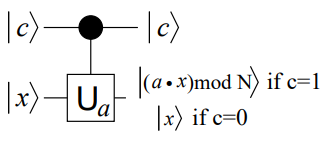
\includegraphics[scale=0.8]{c-Ugate.PNG}
\centering
\end{figure}
Aufgrund der Komplexität dieser Gatter erfolgt der Aufbau schrittweise.
\subsubsection{Adder-Gate}
Ein wichtiger Bestandteil ist das Adder-Gate, dessen Zweck darin besteht,
den Wert \(a\) zu einem Quantenregister hinzuzufügen.
Da \(a\) eine klassische Zahl darstellt, ist es möglich,
die Addition ohne die Verwendung eines zusätzlichen Quantenregisters durchzuführen.
Der Trick besteht darin, die Addition in der Fourier-Basis durchzuführen,
anstatt dies in der Standard- oder Computational-Basis zu tun,
wie es bei einem klassischen Volladdierer der Fall ist.
In Abbildung~\ref{fig:Quantum-Addition} ist anhand des \(\phi\) des Quantenregister \(\ket{\phi(a_n)}\) erkennbar,
dass sich dieses in der Fourier-Basis befindet.
Anschließend wird auf das Quantenregister \(\ket{\phi(a_n)}\) kontrolliert eine Phasenverschiebung übertragen,
abhängig vom Inhalt des klassischen Registers \(\ket{b_n}\).
Dieses Vorgehen entspricht der Addition in der Fourier-Basis und ermöglicht es,
die benötigten Qubits von \(3n\) auf \(n\) zu reduzieren.
\begin{figure}[h]
\caption{Quantum-Addition~\autocite{draper2000addition}}
\label{fig:Quantum-Addition}
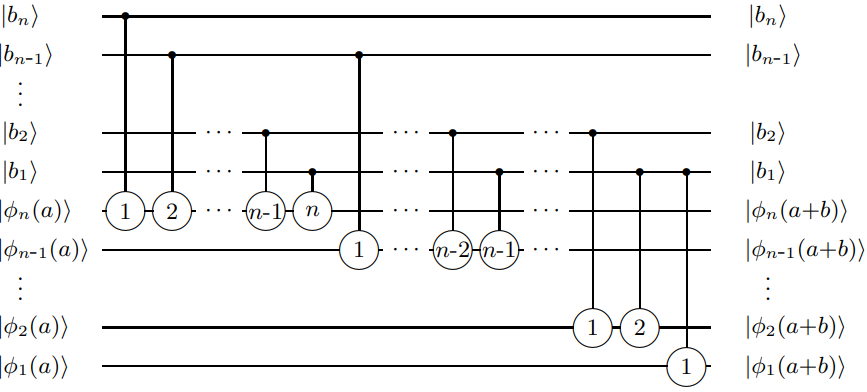
\includegraphics[scale=0.4]{Quantum-Addition.PNG}
\centering
\end{figure}
\subsubsection{Implementierung}
Erklärung Umsetzung Qiskit- also wie wurden die Phasegatter realisiert bzw vorgerechnet. 



%------------------------------------------------

\subsection{Ausblick}


%----------------------------------------------------------------------------------------
%	 REFERENCES
%----------------------------------------------------------------------------------------

\printbibliography % Output the bibliography

%----------------------------------------------------------------------------------------
\end{document}

